% !TEX program = xelatex
\documentclass[12pt]{ctexart}
\usepackage{multirow,graphicx,textcomp,bigstrut,float,syntonly,amsmath,amsfonts,amssymb,etoolbox,indentfirst,bm,subfigure}
\usepackage{amsmath}
\usepackage{amssymb}
\usepackage{algorithm}
\usepackage{algorithmicx}
\usepackage{algpseudocode}
\CTEXoptions[today=old]
\CTEXsetup[format={\Large\bfseries}]{section}
\title{Rule Based Classification of SPE and IFE report}
\author{Li Hanyu}
\date{\today}
\begin{document}
\maketitle
\newpage
\section{Labels}
\par Every combination of SPE and IFE will be transformed into a 12-dimension 0-1 vector like [1, 0, 1, 0, 0, 0, 0, 1, 0, 0, 0, 1]. Above is the label of IgG $\lambda$ situation.

\begin{tabular}{|c|c|c|c|c|c|c|}
    \hline
    component&1&2&3&4&5&6\\
    \hline
    related columns&IgG,$\kappa$&IgG,$\lambda$&IgA,$\kappa$&IgA,$\lambda$&IgM,$\kappa$&IgM,$\lambda$\\
    \hline
    wheather 0 or 1&\multicolumn{6}{|c|}{1 if obvious peaks have same position}\\
    \hline
    \hline
    component&0&7&8&9&10&11\\
    \hline
    related columns&overall&IgG&IgA&IgM&$\kappa$&$\lambda$\\
    \hline
    wheather 0 or 1&only 0 when 7-11 is 0&\multicolumn{5}{|c|}{1 if obvious peaks are detected}\\
    \hline
    \end{tabular}
\begin{enumerate}
    \item The first component is the overall judgement(1 if abnormal and 0 if normal).
    \item The next 6 components are the links between heavy chain(IgG, IgA, IgM) and light chain($\kappa$ and $\lambda$). For example, if IgG and $\lambda$ has the same peak position, then the third component will be 1, because the order is:G$\kappa$, G$\lambda$, A$\kappa$, A$\lambda$, M$\kappa$, M$\lambda$.
    \item The last 5 components are wheather hard and strong edges(obvious peak) are detected in the corresponding column of IFE.
\end{enumerate}
\section{Classification Rules}
\subsection{Peak Detection Method(can only tackle single peak situation)}
\par After reading in a picture of SPE and IFE like:(IgG and $\lambda$ situation)
\begin{figure}[H]
    \centering
    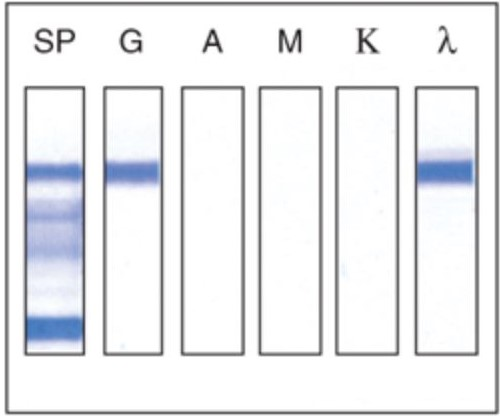
\includegraphics[width=0.5\linewidth]{gl.jpg}
\end{figure}
cv2.fastNlMeansDenoising are applied to every column of the electrophoresis result. Six density plots are then analysed according to the columns.
\begin{figure}[H]
    \centering
    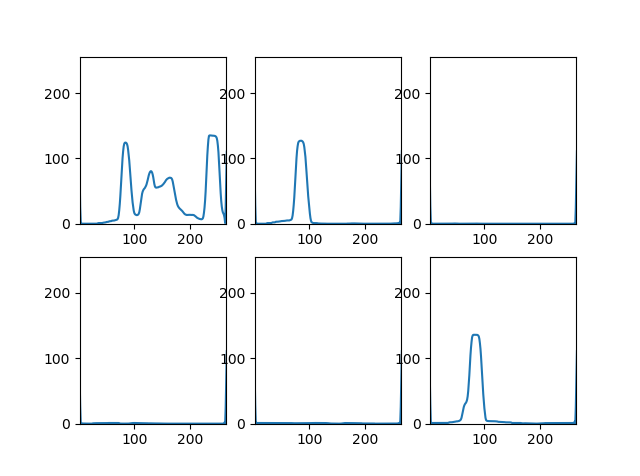
\includegraphics[width=0.5\linewidth]{IgG-lambda.png}
\end{figure}
Afterwards, we apply cv2.Sobel(take derivative) to the density plots and find the max, max position, min, min position of the derivative curve. The column will be labelled as abnormal in the last five components of the label if the $\frac{max(f')+|min(f')|}{2}$ is higher than a formerly set threshold $t_1$. The link between certain kinds of heavy and light chain will be noticed if the difference of the peak position (which is determined by the mean of max position and min position) of the two chains are less than another threshold $t_2$, and both $\frac{max(f')+|min(f')|}{2}$ are higher than threshold $t_3$.
\subsection{Gaussian Mixture Model Methods}
\par Using derivative and second order derivative can lead to troublesome results sometime. In addition, coding a edge detection based model that is capable of dealing multiple peaks takes long time and hard work. On contrast, extracting peak information using Gaussian mixture model is both comparatively simple and effective.
\par Gaussian mixture model is an iteritive aIgorithm using estimation maximization. It assumes that the data is the weighted conbination of several Gaussian distribution. The number of the components(Gaussian distribution) are usually set manually. Specifically, we can view the density plot of the gel electrophoresis as a sample, where the sample number of certain position is in direct proportion to the density of that position. Thus, ideally the density plot will be divide in to seperate components of Gaussian distribution which approximates the concentration of charged protains(peaks).
\par After we find the proper decomposition of the density plot(examples in section 3.2), we can use our prior knowledge to match peaks in different columns and determine if a peak indicates monoclonal component.
\par Firstly we try to preprocess the peak information provided by the GMM(Gaussian Mixture Model). GMM divide the density plot to several distinct Gaussian components, therefore it is possible that it may wrongly treat one polyclonal peak as the sum of two sharp(i.e. monoclonal) peaks. We can name the situation as "far overlap". For instance the 1 and 4 column in the picture below.
\begin{figure}[H]
    \centering
    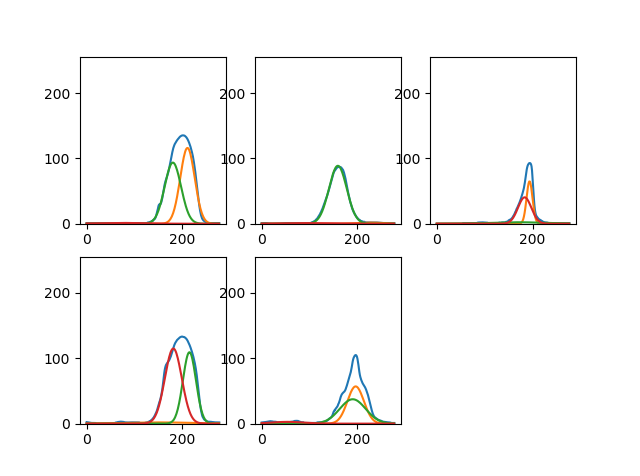
\includegraphics[width=0.5\linewidth]{f.png}
\end{figure}
\par However, a sharp peak in the middle of a polyclonal background is also a tricky problem. If the mean of the background peak and the sharp peak is almost the same, the GMM will give us unsatisfying result where the extracted sharp peak is not as sharp as we think. For instance column 5 in the picture above. We can name this case "near overlap".
\par To sum up, the classification rules should be able to identify near and far overlap and of course stay robust when countering these cases. Identifying is easy because all we need to do is considering the means of every pair of components in one column for each column. Hence, the rule has two steps: preprocessing and classifying. In preprocessing step, we supress the far overlap components so that each one of them will be considered normal. Of course when the weight difference or the variance difference is too large this mechanism will not be trigered. At the same time, the weight of each peak of the near overlap case will be replaced by the sum of the weights. In the classifying step we can consider every components with the all the components in the rest of the columns, and the rules are similar with the peak detection method in the column matching part, but here we use $t=\frac{Variance}{n\_samples*weight}$ as the Identifying value. If t is lower than a manually set threshold than the classifier will lable it as abnormal.
\section{Instances}
\subsection{Peak Detection Methods}
For normal and polyclonal increase instances:
\subsubsection{normal}
\begin{figure}[H]
    \centering
    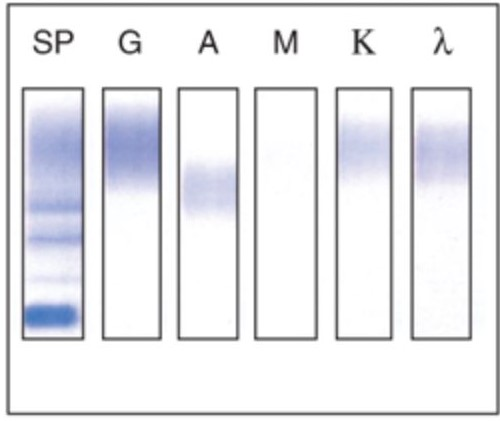
\includegraphics[width=0.5\linewidth]{no.jpg}
\end{figure}
\begin{figure}[H]
    \centering
    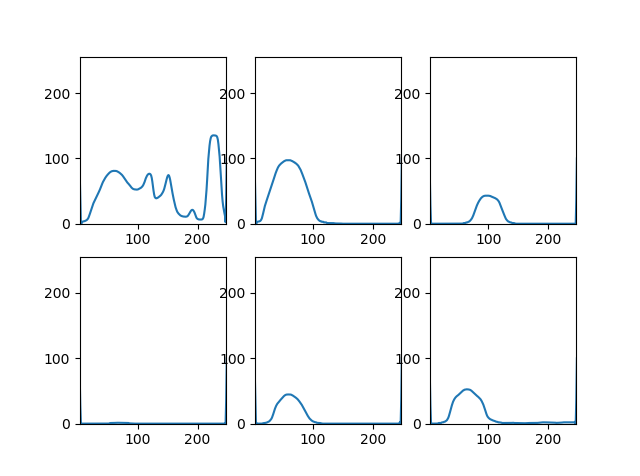
\includegraphics[width=0.5\linewidth]{normal.png}
\end{figure}
label: [0, 1, 1, 0, 0, 0, 0, 0, 0, 0, 0, 0]
\subsubsection{polyclonal increase}
\begin{figure}[H]
    \centering
    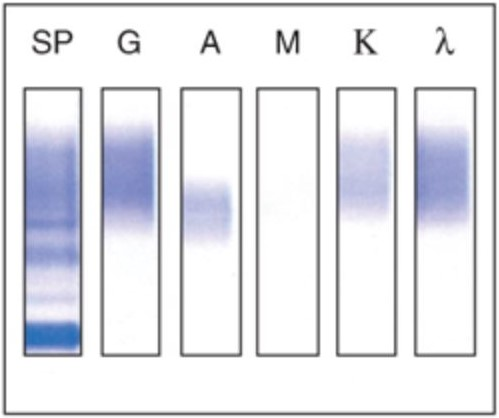
\includegraphics[width=0.5\linewidth]{pr.jpg}
\end{figure}
\begin{figure}[H]
    \centering
    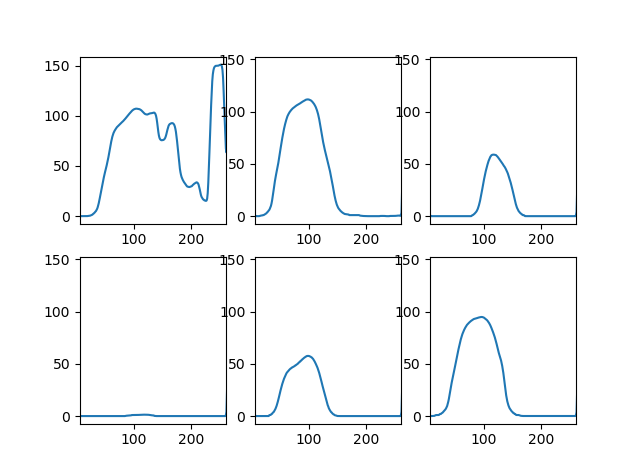
\includegraphics[width=0.5\linewidth]{polyclonal-increase.png}
\end{figure}
label:[0, 1, 1, 0, 0, 0, 0, 0, 0, 0, 0, 0]
\subsection{Gaussian Mixture Model Methods}
\subsubsection{IgM+, Lambda+:}
\begin{figure}[H]
    \centering
    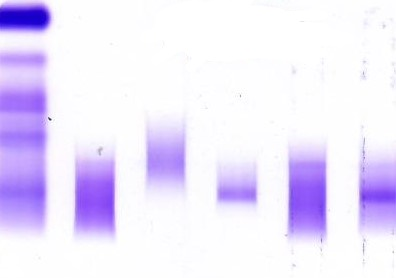
\includegraphics[width=0.5\linewidth]{f1.jpg}
\end{figure}
\begin{figure}[H]
    \centering
    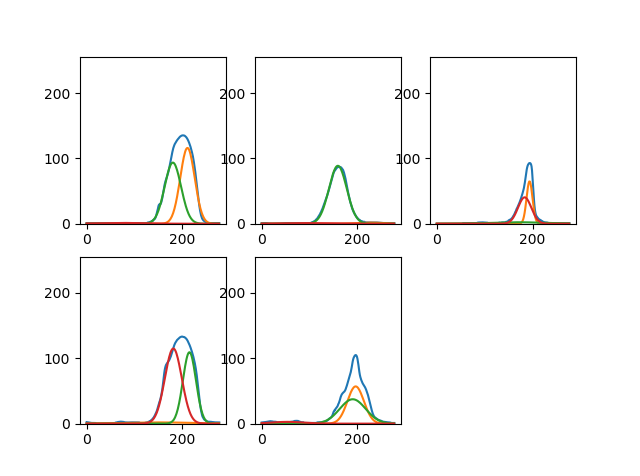
\includegraphics[width=0.8\linewidth]{f.png}
\end{figure}
label:[1,0,0,0,0,0,1,0,0,1,0,1]
\subsubsection{IgG+, Kappa+; IgA+, Kappa+; IgM+, Kappa+}
\begin{figure}[H]
    \centering
    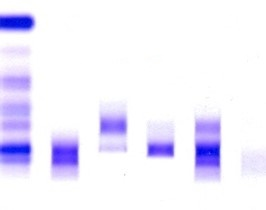
\includegraphics[width=0.5\linewidth]{l1.jpg}
\end{figure}
\begin{figure}[H]
    \centering
    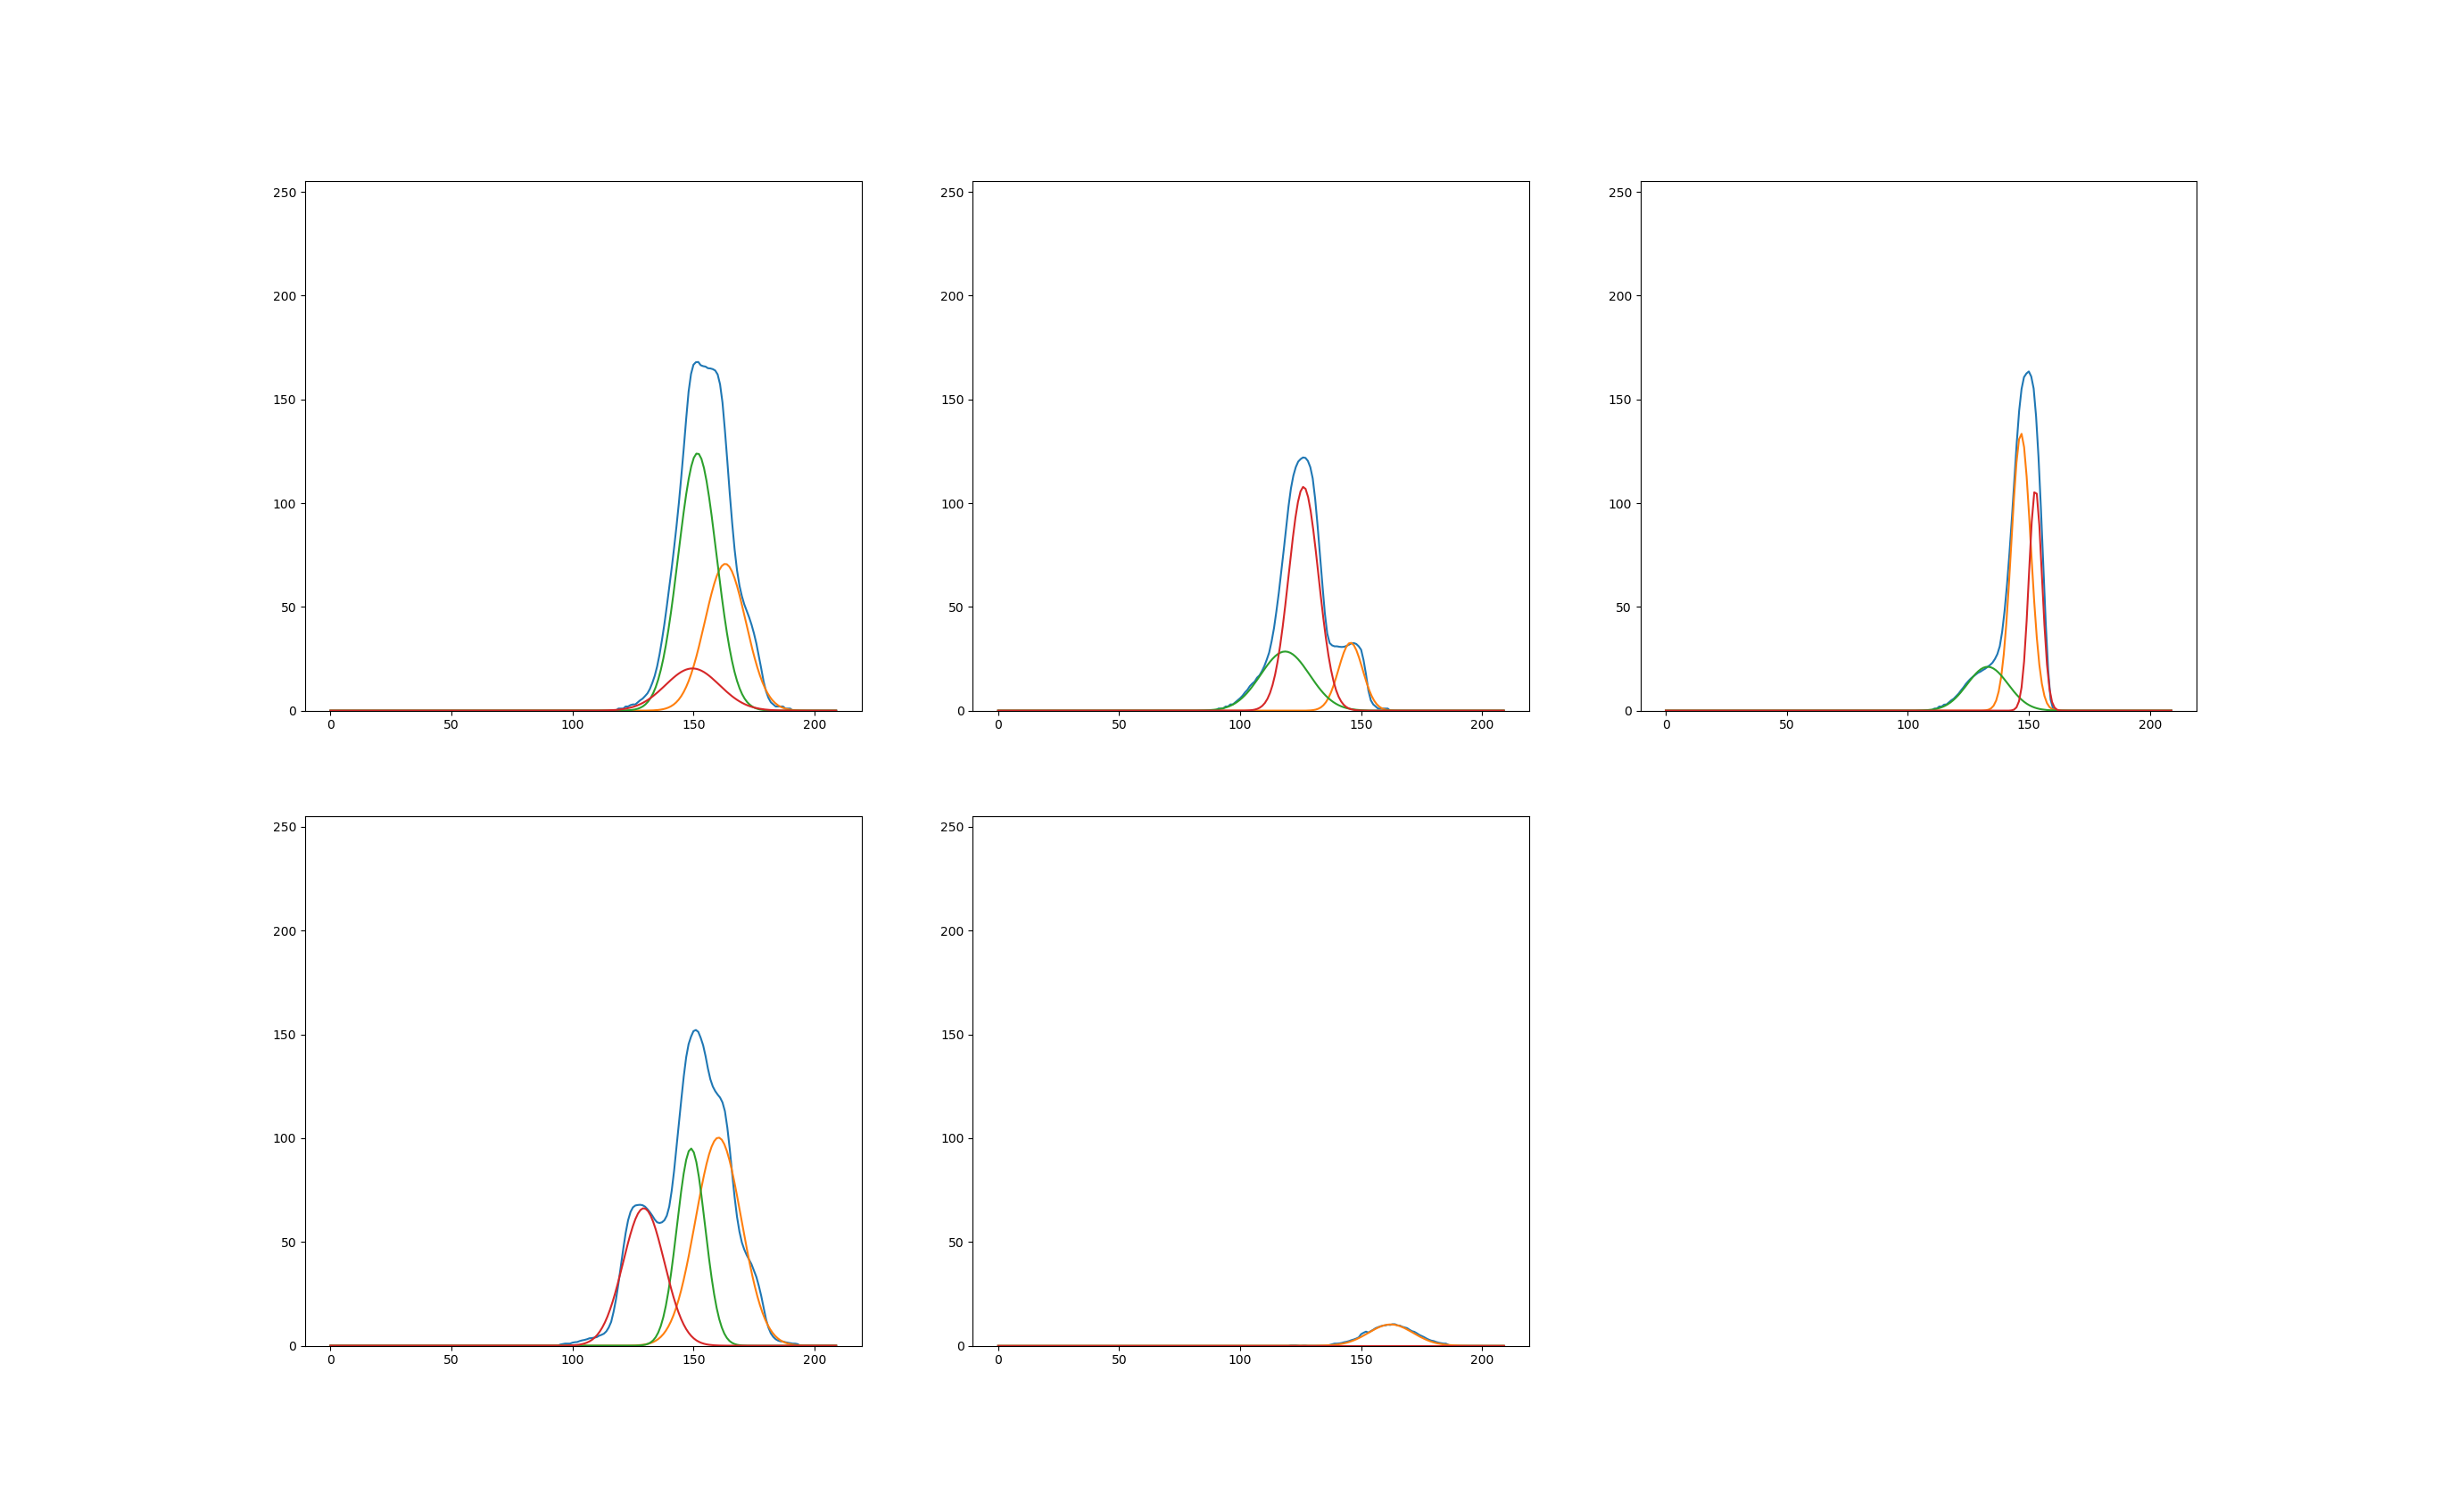
\includegraphics[width=0.8\linewidth]{l.png}
\end{figure}
label:[1,1,0,1,0,1,0,1,1,1,1,0]
\end{document}